\noindent
{\color{stewartblue}\textbf{LỜI GIẢI}}\quad Ta có thể ước tính giá trị của đạo hàm tại bất kỳ giá trị nào của $x$ bằng cách vẽ tiếp tuyến tại điểm $(x, f(x))$ và ước tính hệ số góc của nó. Chẳng hạn, với $x = 3$ ta vẽ một tiếp tuyến tại điểm $P$ trong Hình 2 và ước lượng hệ số góc của nó xấp xỉ bằng $-\frac{2}{3}$. (Chúng ta đã vẽ một tam giác để hỗ trợ việc ước tính hệ số góc.) Do đó $f'(3) \approx -\frac{2}{3} \approx -0{,}67$, điều này cho phép ta chấm điểm $P'(3; -0{,}67)$ trên đồ thị của $f'$ ngay phía dưới điểm $P$. (Hệ số góc của đồ thị hàm số $f$ trở thành giá trị $y$ trên đồ thị hàm số $f'$.)

\vspace{0.8em}
\noindent
\marginpar{\vspace{100pt}\textbf{\small HÌNH 2}}
\begin{center}
  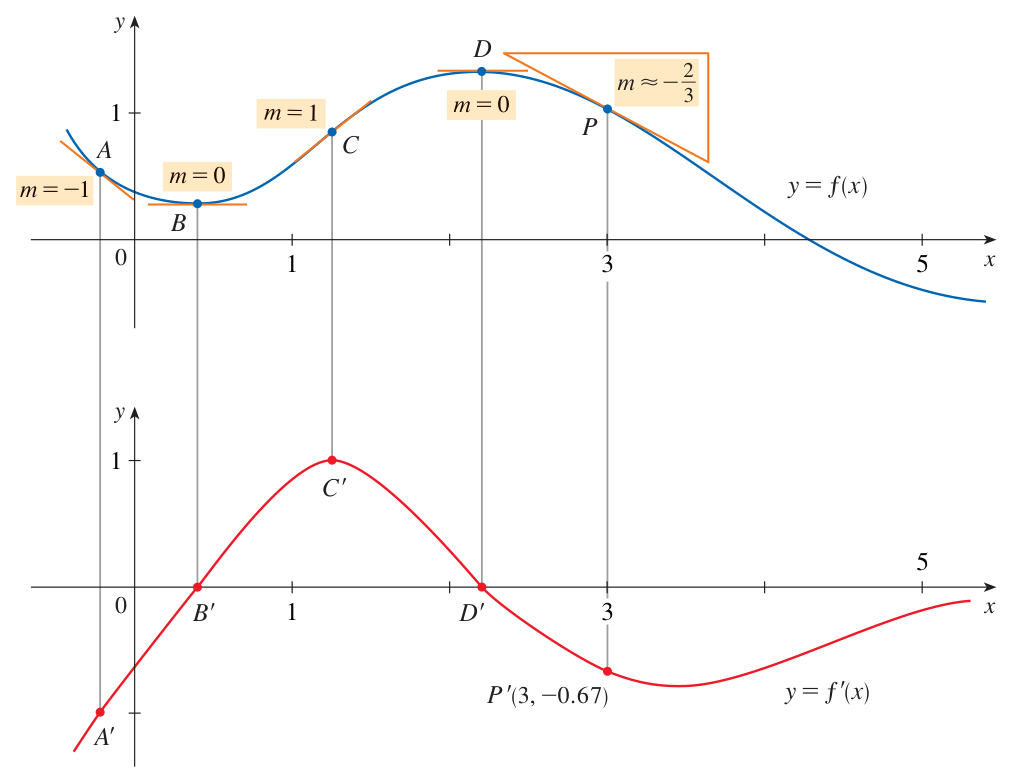
\includegraphics[width=0.88\linewidth]{images/p0189_fig1.png}
\end{center}
\vspace{0.5em}

\noindent
Hệ số góc của tiếp tuyến được vẽ tại $A$ có vẻ bằng khoảng $-1$, vì vậy ta chấm điểm $A'$ với tung độ $y = -1$ trên đồ thị của $f'$ (ngay bên dưới điểm $A$). Các tiếp tuyến tại $B$ và $D$ đều nằm ngang, do đó đạo hàm tại đó bằng 0 và đồ thị của $f'$ cắt trục hoành $x$ (nơi $y = 0$) tại các điểm $B'$ và $D'$, ngay bên dưới $B$ và $D$. Giữa $B$ và $D$, đồ thị của $f$ dốc nhất tại $C$ và tiếp tuyến tại đó có vẻ có hệ số góc bằng 1, do đó giá trị lớn nhất của $f'(x)$ giữa $B'$ và $D'$ là 1 (tại $C'$).

\vspace{0.6em}
\noindent
Lưu ý rằng giữa $B$ và $D$ các tiếp tuyến đều có hệ số góc dương, vì vậy $f'(x)$ mang giá trị dương tại khoảng này. (Đồ thị của $f'$ nằm phía trên trục $x$.) Nhưng ở phía bên phải của điểm $D$, các tiếp tuyến có hệ số góc âm, do đó $f'(x)$ mang giá trị âm ở phần này. (Đồ thị của $f'$ nằm phía dưới trục $x$.)\hfill{\color{stewartblue}\rule{1.3ex}{1.3ex}}

\vspace{1.5em}
\noindent
{\color{stewartblue}\textbf{VÍ DỤ 2}}
\begin{enumerate}[label=(\alph*),leftmargin=2em,itemsep=2pt,topsep=3pt]
  \item Nếu $f(x) = x^3 - x$, hãy tìm công thức cho $f'(x)$.
  \item Minh họa công thức này bằng cách so sánh đồ thị của $f$ và $f'$.
\end{enumerate}

\vspace{0.6em}
\noindent
{\color{stewartblue}\textbf{LỜI GIẢI}}
\begin{enumerate}[label=(\alph*),leftmargin=2em,itemsep=2pt,topsep=3pt]
  \item Khi sử dụng Phương trình 2 để tính đạo hàm, chúng ta cần nhớ rằng biến số
\end{enumerate}
